% mycsrf 'for beeing included' snippet template
%
% (c) Karsten Reincke, Frankfurt a.M. 2012, ff.
%
% This text is licensed under the Creative Commons Attribution 3.0 Germany
% License (http://creativecommons.org/licenses/by/3.0/de/): Feel free to share
% (to copy, distribute and transmit) or to remix (to adapt) it, if you respect
% how you must attribute the work in the manner specified by the author(s):
% \newline
% In an internet based reuse please link the reused parts to mycsrf.fodina.de
% and mention the original author Karsten Reincke in a suitable manner. In a
% paper-like reuse please insert a short hint to mycsrf.fodina.de and to the
% original author, Karsten Reincke, into your preface. For normal quotations
% please use the scientific standard to cite
%

\section{Prozessgüte und Prozessreife einzelner Ketten}

Wir werden in den folgenden Abschnitten die Ergebnisse unserer Tests nur
summarisch protokollieren. Trotzdem ist die Reproduzierbarkeit und
Überprüfbarkeit auf folgende Weise gewährleistet:

\begin{itemize}
  \item In den Quellen zu diesem Text\footcite[vgl.][\nopage wp]{Reincke2019a}
  findet sich auch der Ordner \texttt{chain-evaluation}. Sofern nicht von unser
  Distribution generell bereitgestellt, enthält dieser Ordner alle
  IO-(Zwischen)-Ergebnisse und alle Tools resp. Makefiles, die auf den
  definierten Wegen benötigt resp. erzeugt werden.
  \item Als erstes haben wir in jedem Frontend -- sei es per Import\footnote{die
  entsprechende XML Datei ist beigelegt}, sei es manuell -- in etwa folgende
  Eingabe zu erzeugen versucht:
  \begin{center}
    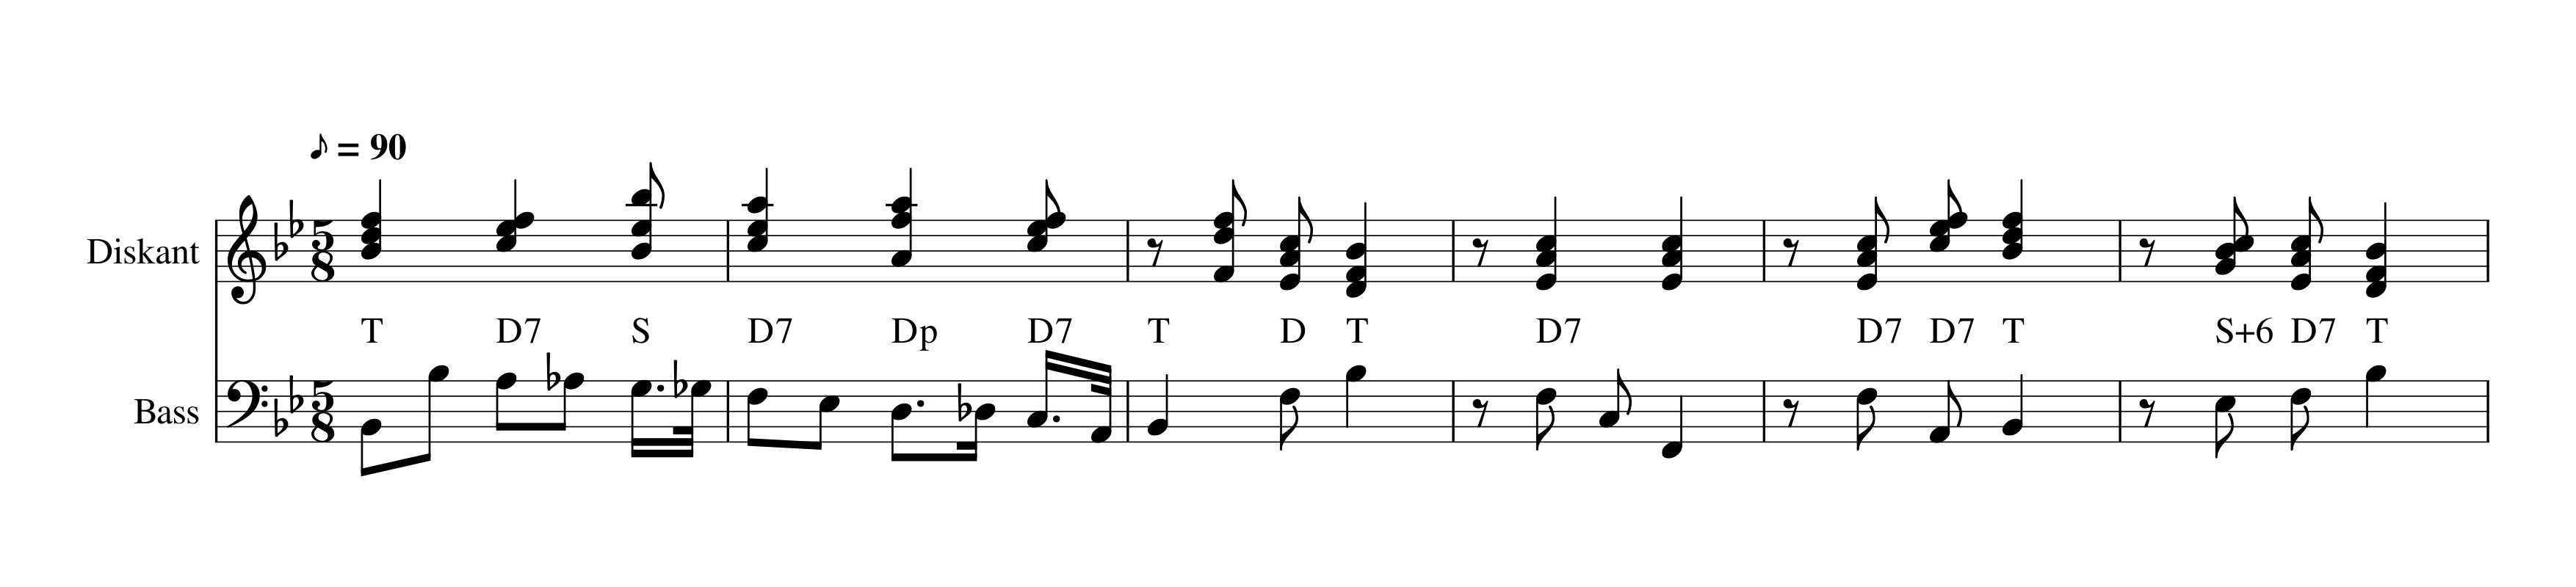
\includegraphics[width=0.9\textwidth]{frontends/musescore/cadenca3-musescore-300dpi.png}
  \end{center}
  Wir wissen ja bereits, dass die ausgefeilte Harmoniedokumentation in keinem
  Frontend möglich ist. Wir erwarten technisch aber, dass die vereinfachte
  Darstellung problemlos ins Backend übertragen wird und -- bei MusiX\TeX\ und
  LilyPond -- manuell durch die besseren Versionen ersetzbar ist, also
  bei MusiX\TeX\ durch \acc{harmony}-Konstrukte und bei LilyPond durch die unser
  kleinen Zusatzbibliothek.
  \item Danach haben wir in jedem Fronted alle möglichen Exporte angestoßen und
  die Ergebnisse in einem Ordner \texttt{from-frontend-to} abgelegt.
  \item Für jeden Weg, der vom Fontend aus gegangen werden kann, gibt es im
  Frontendordner einen Ordner mit der entsprechenden Nummer.
  \item Wird der Output des Frontends gemäß der Wegdefinition direkt als Input für
  das Backend verwendet, findet sich im Wegordner ein entsprechendes \LaTeX- und
  Makefile und die so generierte PDF-Datei.
  \item Wird der Output des Frontends dagegen einem Konverter vorlegt, enthält
  der Wegeordner auch den Output des Konverters. \LaTeX- und Makefile
  operieren dann auf und mit diesen Daten.
  \item Dort, wo das entsprechende Frontend oder der Konverter nicht von unserer
  Referenzdistribution\footnote{Ubuntu 18.04} bereitgestellt wird, haben wir die
  entsprechenden Pakete beigelegt.
\end{itemize}

Mit diesen Materialien haben wir die folgenden Ergebnisse erzeugt.

\subsection{w01: Easy\-ABC \ra\ \LaTeX+ABC (0.8/0.56)}\label{w01}

Die aus Easy\-ABC als \acc{abc}-Code exportierte Referenzkadenz III kann manuell
in das \LaTeX-Backend kopiert werden, was daraus -- technisch gesehen --
reibungslos die korrespondierende PDF-Datei erzeugt. Den Output des Frontends
separat zu halten und mit \LaTeX-Mitteln per \texttt{input} automatisiert zu
integrieren, scheitert jedoch. Die freie Verwendung des Zeichen \texttt{\$} im
importierten Code verwirrt zudem das Syntaxhighlighting von wenigstens einigen
Editoren. Schließlich wird die vorgegebene Tempoangabe \texttt{\Acht=90} während
des Exports/Imports in \texttt{\Vier=45} umgewandelt. Das ist bei einem
\texttt{5/8}-Takt nicht sinnvoll und muss manuell korrigiert werden. Das
schließlich erzeugbare Ergebnis ist allerdings graphisch perfekt.

Man muss also konstatieren, dass die Konvertierung als Prozess zwar
\acc{stolpert}, aber \acc{exzellente} Ergebnisse erzeugt. Damit ergibt sich
eine Prozessgüte von \texttt{0.8} und eine normierte Prozessreife von
\texttt{((4+3-0)*0.8)/10=0.56}.

\subsection{w02: Easy\-ABC \ra\ xml2abc \ra\ \LaTeX+ABC: (0.8/0.48)}\label{w02}

Der Konverter \acc{xml2ab} wird mit \acc{EasyABC} mitgeliefert.\footnote{Im
Sourcecode-Ordner zu starten mit \texttt{python xml2abc}} Er nimmt die aus
Easy\-ABC als \acc{xml}-Code exportierte Referenzkadenz III und konvertiert sie
in \acc{abc}-Code. Dieser kann seinerseits manuell in das \LaTeX-Backend kopiert
werden, damit es -- technisch gesehen -- reibungslos die korrespondierende,
graphisch \acc{exzellente} PDF-Datei erzeugt.\footnote{Materialien dazu unter
\ra\
\texttt{mycsrf/examples/musicology.de/chain-evaluation/from-EasyABC-to/w02}}

Dabei treten jedoch die gleichen Irritation auf, wie bei der direkten Nutzung
der aus dem Frontend gesicherten \acc{abc}-Datei:\footnote{\ra\ S.\pageref{w01}}
Die \acc{ABC}-Outputdatei kann nicht mit \LaTeX-Mitteln inkludiert werden, die
freie Verwendung von \texttt{\$} verwirrt manche Editoren, und die Tempoangabe
muss manuell auf \texttt{\Acht=90} zurückgesetzt werden.

Auch hier ist also festzuhalten, dass die Konvertierung als Prozess zwar
\acc{stolpert}, aber nichtsdestotrotz \acc{exzellente} Ergebnisse erzeugt. Damit
ergibt sich eine Prozessgüte von \texttt{0.8} und eine normierte Prozessreife
von \texttt{((4+3-1)*0.8)/10=0.48}.

\subsection{w04: Easy\-ABC \ra\ abc2ly \ra\ ly2abc \ra\ \LaTeX+ABC: (1.0)}\label{w04}

\acc{abc2ly} wird von \acc{Lilypond} als Tool mitgeliefert und über die
Kommandozeile aufgerufen.\footnote{\ra\
\href{http://lilypond.org/doc/v2.19/Documentation/usage/invoking-abc2ly.de.html}
{http://lilypond.org/doc/v2.19/Documentation/usage/invoking-abc2ly.de.html}} Das
Kommando \texttt{abc2ly cadenca3-from-easyabc.abc} nimmt die \acc{abc}-Datei
und erzeugt die korrespondierende Lilypond-Datei \texttt{cadenca3-from-easyabc.ly}.

Unglücklicherweise meldet die Konvertierung selbst schon mit den Worten
\acc{Huh? Don't understand}, dass etwas nicht korrekt läuft. Die generierte
\acc{LilyPond}-Datei kann zwar noch problemlos in die \LaTeX-Datei eingebunden
werden und mit dem LilyPond adäquate Makefile in eine PDF-Datei umgewandelt 
werden. Das Ergebnis ist aber kaum noch als eine 'Varianten' der
Referenzkadenz III zu erkennen. Dasselbe Bild zeigt sich, wenn man das Ergebnis
der Konversion mit dem \acc{LilyPond}-Editor \acc{Frescobaldi} öffnet. erst
auf den 3. Blick erkennt man  noch Zusammenhänge.

Hier also läuft der Konvertierungsprozess zwar technisch reibungslos, dass Ergebnis
aber ist \acc{inakzeptabel}. Damit
ergibt sich eine Prozessgüte von \texttt{0} und eine normierte Prozessreife
von \texttt{((4+3-2)*0)/10=0.0}.


\subsection{w05: Easy\-ABC \ra mxml2ly \ra\ ly2abc \ra\ \LaTeX+ABC: (1.0)}

5

\subsection{w06: Easy\-ABC \ra xml2ly \ra\ ly2abc \ra\ \LaTeX+ABC: (1.0)}

6

\subsection{w07: Rose\-garden \ra\ xml2abc \ra\ \LaTeX+ABC: (1.0)} 

7

\subsection{w08: Rose\-garden \ra\ mxml2abc \ra\ \LaTeX+ABC: (1.0)} 

8

\subsection{w09: Rose\-garden \ra\ mxml2ly \ra\ ly2abc \ra\ \LaTeX+ABC: (1.0/1.0)} 

9

\subsection{w10: Rose\-garden \ra\ xml2ly \ra\ ly2abc \ra\ \LaTeX+ABC: (1.0)} 

10

\subsection{w11: Muse\-Score \ra\ xml2abc \ra\ \LaTeX+ABC: (1.0)} 

11

\subsection{w12: Muse\-Score \ra\ mxml2abc \ra\ \LaTeX+ABC: (1.0)}

12

\subsection{w13: Muse\-Score \ra\ mxml2ly \ra\ ly2abc \ra\ \LaTeX+ABC: (1.0)} 

13

\subsection{w14: Muse\-Score \ra\ xml2ly \ra\ ly2abc \ra\ \LaTeX+ABC: (1.0)}

14

\subsection{w15: Denemo \ra\ xml2abc \ra\ \LaTeX+ABC: (1.0)}

15

\subsection{w16: Denemo \ra\ mxml2abc \ra\ \LaTeX+ABC: (1.0)} 

16

\subsection{w17: Denemo \ra\ mxml2ly \ra\ ly2abc \ra\ \LaTeX+ABC: (1.0)} 

17

\subsection{w18: Denemo \ra\ xml2ly \ra\ ly2abc \ra\ \LaTeX+ABC: (1.0)} 

18

\subsection{w19: Canorus \ra\ xml2abc \ra\ \LaTeX+ABC: (1.0)} 

19

\subsection{w20: Canorus \ra\ mxml2abc \ra\ \LaTeX+ABC: (1.0)} 

20

\subsection{w21: Canorus \ra\ mxml2ly \ra\ ly2abc \ra\ \LaTeX+ABC: (1.0)} 

21

\subsection{w22: Canorus \ra\ xml2ly \ra\ ly2abc \ra\ \LaTeX+ABC: (1.0)} 

22

\subsection{w23: Texteditor \ra\ \LaTeX+ABC: (1.0)}

23

\subsection{w24: EasyABC \ra\ abc2mtex \ra\ \LaTeX+Musix\TeX: (1.0)} 

24

\subsection{w25: EasyABC \ra\ mxml2pmx \ra\ pmxab \ra\ \LaTeX+Musix\TeX: (1.0)} 

25

\subsection{w26: Rosegarden \ra\ mxml2pmx \ra\ pmxab \ra\ \LaTeX+Musix\TeX: (1.0)}

26

\subsection{w27: MuseScore \ra\ mxml2pmx \ra\ pmxab \ra\ \LaTeX+Musix\TeX: (1.0)}

27

\subsection{w28: Denemo \ra\ mxml2pmx \ra\ pmxab \ra\ \LaTeX+Musix\TeX: (1.0)} 

28

\subsection{w29: Canorus \ra\ mxml2pmx \ra\ pmxab \ra\ \LaTeX+Musix\TeX: (1.0)} 

29

\subsection{w30: Texteditor \ra\ \LaTeX+Musix\TeX: (1.0)}

30

\subsection{w31: Texteditor \ra\ pmxab \ra\ \LaTeX+Musix\TeX: (1.0)}

31

\subsection{w32: Easy\-ABC \ra xml2ly \ra\ Elysium \ra\ \LaTeX+LilyPond: (1.0)} 

32

\subsection{w33: Easy\-ABC \ra mxml2ly \ra\ Elysium \ra\ \LaTeX+LilyPond: (1.0)} 

33

\subsection{w34: Easy\-ABC \ra xml2ly \ra\ Frescobaldi \ra\ \LaTeX+LilyPond: (1.0)}

34

\subsection{w35: Easy\-ABC \ra mxml2ly \ra\ Frescobaldi \ra\ \LaTeX+LilyPond: (1.0)} 

35

\subsection{w36: Rosegarden \ra xml2ly \ra\ Elysium \ra\ \LaTeX+LilyPond: (1.0)}

36

\subsection{w37: Rosegarden \ra mxml2ly \ra\ Elysium \ra\ \LaTeX+LilyPond: (1.0)}

37

\subsection{w38: Rosegarden \ra xml2ly \ra\ Frescobaldi \ra\ \LaTeX+LilyPond: (1.0)}

38

\subsection{w39: Rosegarden \ra mxml2ly \ra\ Frescobaldi \ra\ \LaTeX+LilyPond: (1.0)}

39

\subsection{w40: MuseScore \ra xml2ly \ra\ Elysium \ra\ \LaTeX+LilyPond: (1.0)}

40

\subsection{w41: MuseScore \ra mxml2ly \ra\ Elysium \ra\ \LaTeX+LilyPond: (1.0)}

41

\subsection{w42: MuseScore \ra xml2ly \ra\ Frescobaldi \ra\ \LaTeX+LilyPond: (1.0)} 

42

\subsection{w43: MuseScore \ra mxml2ly \ra\ Frescobaldi \ra\ \LaTeX+LilyPond: (1.0)} 

43

\subsection{w44: Denemo \ra xml2ly \ra\ Elysium \ra\ \LaTeX+LilyPond: (1.0)} 

44

\subsection{w45: Denemo \ra mxml2ly \ra\ Elysium \ra\ \LaTeX+LilyPond: (1.0)} 

45

\subsection{w46: Denemo \ra xml2ly \ra\ Frescobaldi \ra\ \LaTeX+LilyPond: (1.0)}

46

\subsection{w47: Denemo \ra mxml2ly \ra\ Frescobaldi \ra\ \LaTeX+LilyPond: (1.0)}

47

\subsection{w48: Canorus \ra xml2ly \ra\ Elysium \ra\ \LaTeX+LilyPond: (1.0)}

48

\subsection{w49: Canorus \ra mxml2ly \ra\ Elysium \ra\ \LaTeX+LilyPond: (1.0)}

49

\subsection{w50: Canorus \ra xml2ly \ra\ Frescobaldi \ra\ \LaTeX+LilyPond: (1.0)}

50

\subsection{w51: Canorus \ra mxml2ly \ra\ Frescobaldi \ra\ \LaTeX+LilyPond: (1.0)}

51

\subsection{w52: Text-Editor \ra\ \LaTeX+LilyPond: (1.0)}

52

\subsection{w53: Elysium \ra\ \LaTeX+LilyPond: (1.0)}

53
\subsection{w54: Frescobaldi \ra\ \LaTeX+LilyPond: (1.0)}

54



